
\newpage
\section{Checkpoint 6: Data Handling and Analysis}

\begin{enumerate}

\item [6.1.] This is a data handling exercise and the Raspberry Pi is not required.
Thus this checkpoint is best carried out using the Physics CPlab computers. 
There is a CPlab computer available on every desk in the DAH laboratory.
You can use the following python libraries. \\

\lstinputlisting{../scripts/checkpoint_6a.py}

The LHCb experiment at the Large Hadron Collider at CERN has recorded a sample of muon pairs with invariant masses in the range of 8.5 to 11 GeV/$c^2$. Three clear peaks are observed in this mass spectrum. These correspond to the production of Upsilon mesons, which are bound states of a $b$ and a anti-$b$ quark. These states are known as the $\Upsilon \rm (1S)$, $\Upsilon \rm (2S)$ and $\Upsilon \rm (3S)$ mesons where the $\Upsilon \rm (1S)$ meson is the ground state and the $\Upsilon \rm (2S)$  and $\Upsilon \rm (3S)$  states are radial excitations (for LHCb paper, see {DOI: 10.1007/JHEP06(2013)064).}

\begin{center}
    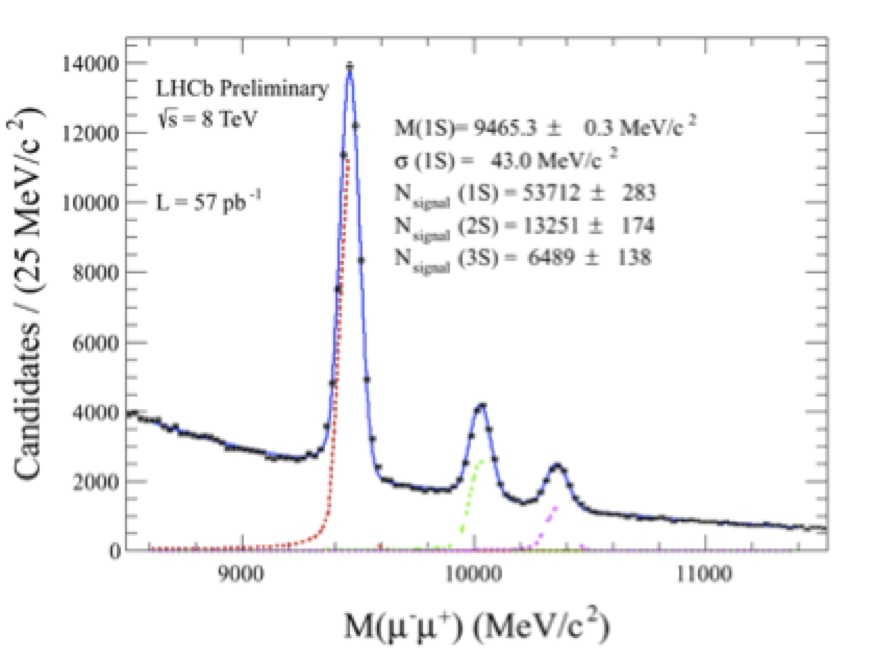
\includegraphics[width=9cm]{figs/mu-pair-mass}
\end{center}

Download the file upsilons-mass-xaa.txt from the DAH Dropbox, which contains the invariant masses of a large number of muon pairs in units of GeV/$c^2$ in text format. Write a python script that reads the data from this file and plots a histogram of all the masses, choosing a reasonable bin width. Always label plots correctly with title and axes and save these to a file.
[Hint: The bin width should be chosen such that each of the three peaks is clearly resolved and represented by a sufficient number of bins for analysis.]

\hfill [2 marks]


\item [6.2.] Determine the masses of the three particles by determining the bins with the highest number of entries in the peak regions. Divide the histogram into three peak regions and write a local peak finding method for this part.
What are the mass differences between the $\Upsilon \rm (2S)$ and $\Upsilon \rm (3S)$ states with respect to the $\Upsilon \rm (1S)$ meson? %By inspecting visually the muon-pair mass
%spectrum, determine the Full Width Half Maximum (FWHM) of the $\Upsilon \rm (1S)$ mass peak.

\hfill [2 marks]


\item [6.3.] Determine the mass of the  $\Upsilon \rm (1S)$  meson and its statistical uncertainty. This can be achieved by several methods. First  by looking at the mass spectrum, choose a suitable region around the $\Upsilon \rm (1S)$  mass peak. Calculate the mean, the unbiased variance and standard deviation for the events in this region. Use these values to determine the standard deviation of the mean. Comment on possible biases for this method. 


The mass peaks corresponding to the three $\Upsilon$ mesons can be described 
reasonably well by a Gaussian function, 
$f(x) = \frac{N}{\sigma \sqrt{2\pi}}  \exp{\left( - \frac{(x-/\mu)^2}{2\sigma^2} \right)} $
where $x$ is the invariant mass of the muon pairs, $\mu$ is the mass of the $\Upsilon \rm (1S)$  meson, $\sigma$ is the Gaussian width (mass resolution) and $N$ is the total number of signal events. 
By inspecting visually the muon-pair mass
spectrum, determine the Full Width Half Maximum (FWHM) of the $\Upsilon \rm (1S)$ mass peak.
Assuming a Gaussian signal shape estimate the mass resolution $\sigma$ from the FWHM. %of the $\Upsilon \rm (1S)$  peak. 
Compare this result for the mass resolution of the $\Upsilon \rm (1S)$  peak with the standard deviation in the signal region determined above and comment.

\hfill [3 marks]\\


In the muon-pair mass spectrum define a signal region of width $\pm 150\; {\rm MeV}/c^2$ around the $\Upsilon \rm (1S)$  peak position and determine the number of events $N$ in this region. 
Define an upper and lower sideband region where there are only background events. These sidebands should each be half as wide as the signal region and located at masses equidistant from the $\Upsilon \rm (1S)$  peak position. Assuming that the background is falling linearly with the muon-pair mass, determine the number of background events $B$ in the signal region (below the $\Upsilon \rm (1S)$  mass peak). Perform either a linear least squares fit in the sideband regions or use the sideband subtraction method for this. Determine the number of signal events $S$ in the signal region.

Alternatively, if you know how to perform a fit you may choose fitting the $\Upsilon \rm (1S)$   peak in the mass spectrum for this part.

% Assuming Gaussian statistics for N and using the mass resolution ? determine the statistical error %on the mass of the ?(1S) meson. 
Compare your mass measurement with the Particle Data Group (\url{pdg.lbl.gov}) and comment.
[Hint: The PDG lists the properties of particles. Select "pdgLive - Interactive Listings" followed by "Mesons b anti-b" to find the $\Upsilon \rm (1S)$  meson.]

\hfill [3 marks]

\begin{comment}

6.4. Download the file upsilons-mass-pt-xaa.txt from the DAH Dropbox which, in addition to the masses, also contains the transverse momenta pT of the muon- pairs in units of GeV/c in text format. For an explanation of the transverse momentum, see the LHCb paper, referred to above. Write a python script that reads in these data and plot a histogram of the transverse momenta for all events. Plot a 2-dimensional histogram of pT versus mass for all events, choosing 50 bins in pT and 100 bins in mass.
[Hint (python):]
%# Splitting a line with two strings separated by a blank space line = line.split()
12
[1 mark]

\end{comment}



\end{enumerate}
